\documentclass[11pt,letterpaper]{article}
\usepackage[utf8]{inputenc}
\usepackage[spanish,es-nodecimaldot]{babel}
\usepackage{amsmath}
\usepackage{amsfonts}
\usepackage{amssymb}
\usepackage{color,soul}
\usepackage{textcomp}
\usepackage{stmaryrd}
\usepackage{makeidx}
\usepackage{colortbl}
\usepackage{tocloft}
\renewcommand{\cftsecleader}{\cftdotfill{\cftdotsep}}
\usepackage{rotating}
\usepackage{url}
\usepackage{pdflscape} 
\usepackage{pdfpages}
\usepackage{float}
\usepackage{graphicx}
\usepackage{ marvosym }
\usepackage{pgf,tikz}
\usepackage{mathrsfs}
\usetikzlibrary{arrows}
\usepackage{ mathrsfs }
 \usepackage{array}
\usepackage{longtable}
\newcommand{\justif}[2]{&{#1}&\text{#2}}
\usepackage{listings}
\usepackage{color}
\newcolumntype{L}[1]{>{\raggedright\let\newline\\\arraybackslash\hspace{0pt}}m{#1}}
\newcolumntype{C}[1]{>{\centering\let\newline\\\arraybackslash\hspace{0pt}}m{#1}}
\newcolumntype{R}[1]{>{\raggedleft\let\newline\\\arraybackslash\hspace{0pt}}m{#1}}
\definecolor{dkgreen}{rgb}{0,0.6,0}
\definecolor{gray}{rgb}{0.5,0.5,0.5}
\definecolor{mauve}{rgb}{0.58,0,0.82}
\setboolean{@twoside}{false}
\lstset{frame=tb,
  language=Java,
  aboveskip=3mm,
  belowskip=3mm,
  showstringspaces=false,
  columns=flexible,
  basicstyle={\small\ttfamily},
  numbers=left,
  numberstyle=\tiny\color{gray},
  keywordstyle=\color{blue},
  commentstyle=\color{dkgreen},
  stringstyle=\color{mauve},
  breaklines=true,
  breakatwhitespace=true,
  tabsize=3
}

\usetikzlibrary{graphs,graphs.standard}
\newcommand{\floor}[1]{\lfloor #1 \rfloor}

\usepackage{multicol}

\usepackage{caption}
\usepackage{subcaption}
\begin{document}
\begin{titlepage}
	\centering
	{\scshape\LARGE Universidad Nacional Autónoma de México \par}
	\vspace{1cm}
	{\scshape\Large Facultad de Ciencias\par}
	\vspace{1.5cm}
\begin{center}
		
\includegraphics[scale=.5]{logo.png}
	\end{center}
		\vspace{.8 cm}

	{\huge\bfseries Proyecto Final: \par}
	{\huge\bfseries Traducción al Modelo Relacional \par}
		\vspace{0.5cm}

	{\Large\itshape Flores Martínez Andrés\\
	Vázquez Salcedo Eduardo Eder\\
	Sánchez Pérez Pedro Juan Salvador\\
	Concha Vázquez Miguel\par}
	\vfill
			\vspace{0.5cm}

	Trabajo presentado en cumplimiento con la asignatura de Fundamentos de Bases de Datos impartida por el profesor	\par
	 \textsc{Gerardo Avilés Rosas}\\
	\vspace{0.1cm}
	{\large 12 de enero de 2018\par}
\end{titlepage}

\begin{center}
\tableofcontents
\end{center}

\newpage

\section{Traducción ER a Modelo Relacional}

\subsection{Algoritmo de Traducción}

En el curso aprendimos cómo pasar el modelo entidad-relación al modelo relacional. Lo que se nos recomendó en primer lugar es identificar a las entidades fuertes y especificar sus atributos como parte de la tupla de la relación, subrayando sus atributos llave. Posteriormente, identificar las relaciones con una restricción de cardinalidad muchos-muchos porque estas de entrada crear nuevas relaciones (tablas). Para este tipo de relaciones, tendríamos que añadir los atributos llave de ambas relaciones (en caso de ser binaria) como llaves foráneas con tal de asegurar una integridad de relaciones. \\

En el caso de las relaciones de tipo uno-muchos, lo que se tendría que hacer era agregar la llave de la relación con cardinalidad \textit{uno} a la otra entidad; si era una restricción de participación total de al menos un lado, entonces la podíamos representar a la relación misma con una nueva tabla que incluyera las llaves de cada entidad relacionada como llaves foráneas.\\

Para las relaciones con restricción de cardinalidad uno-uno había varios escenarios:

\begin{itemize}
\item Restricción de participación parcial de ambos lados: Se crea una tabla adicional con las laves de ambas entidades y los atributos de la relación.
\item Restricción de participación total de un lado de la relación: Se incluyen en la tabla correspondiente a la entidad con participación total los atributos de la relación y la llave de la otra entidad.
\item Restricción de participación total de ambos lados: Se incluyen en una sola relación todos los atributos de ambas entidades además de los atributos de la relación.
\end{itemize}

También se nos explicó que los atributos calculados (derivados) no los tendríamos que especificar como parte de las relaciones (tablas), mientras que en el caso de los atributos multivaluados necesitamos crear una nueva relación con el nombre del atributo y como atributo llave el mismo nombre, además de añadir el atributo llave de la entidad como llave foránea.\\


Por último, en los esquemas de especialización había también varios casos:

\begin{itemize}
\item Si la especialización es de completez total, entonces no debíamos agregar una relación para la super-entidad y trabajar directamente con las relaciones de las sub-entidades, agregando el atributo llave de la super-entidad como llave de las sub-entidades, al igual que sus demás atributos.
\item Si la especialización es de completez parcial, entonces se tenía que crear una relación para cada una de las entidades, pero también ``heredar" los atributos y la llave de la super-entidad a las relaciones de las sub-entidades.
\end{itemize} 

Siguiendo este algoritmo y las recomendaciones del profesor Gerardo, consideramos en la siguiente subsección el proceso llevado a cabo para la traducción al modelo de datos relacional.

\subsection{Proceso de Traducción}

De acuerdo con el algoritmo, nos ocupamos primero de las entidades fuertes, para las cuales especificamos sus atributos como partes de la tupla que representa a cada relación y subrayamos en cada caso sus atributos llave. Como en nuestro caso no contamos con entidades débiles, lo hacemos para cada entidad del diagrama ER. Entonces nos queda lo siguiente ---considerando de igual forma que los atributos multivaluados se transforman en tablas y no consideramos a aquellos que sean calculados (derivados) como se explicó anteriormente:

\begin{itemize}
\item {\footnotesize \textbf{Sucursal}(\underline{idSucursal},calle,municipio,colonia,estado,numInterior,numExterior,CP,horaApertura,horaCierre)}
\item \footnotesize{\textbf{SucursalTelefono}(\underline{idSucursal},\underline{telefono})}
\item \footnotesize{\textbf{Historico}(\underline{idHistorico},idProducto,precioPrevio,precioNuevo,fechaActualizacion)}
\item \scriptsize{\textbf{Proveedor}(\underline{RFC},razonSocial,calle,municipio,colonia,estado,numInterior,numExterior,CP,email,inicioRelacion,telefono)}
\item \footnotesize{\textbf{Pedido}(\underline{numPedido},fechaPedido,promocion,preparado,entregado)}
\item \footnotesize{\textbf{ProductoLeyenda}(\underline{idProducto},\underline{leyenda})}
\item \footnotesize{\textbf{Ingrediente}(\underline{idIngrediente},nombre,marca,cantidadExistencia,fechaCaducidad)}
\item \footnotesize{\textbf{Mobiliario}(\underline{idMueble},tipo)}
\item \footnotesize{\textbf{Transporte}(\underline{idTransporte},marca,modelo,tipo)}
\item \footnotesize{\textbf{Licencia}(\underline{código})}
\end{itemize}

Luego, para traducir la jerarquía de especialización que se presenta con la super-entidad \textbf{Persona} y las sub-entidades \textbf{Empleado} y \textbf{Cliente}, notamos que tenemos una especialización total y restricción de disyunción, así que creamos una relación para cada subentidad, incluyendo tanto sus atributos como los de la super-entidad; la llave es la de la super-entidad. Nos quedan entonces:

\begin{itemize}
\item \footnotesize{\textbf{Cliente}(\underline{taquiClave},email,telefono,nombre,apellidoPaterno,apellidoMaterno,calle,municipio,colonia,estado,
numInterior,numExterior,CPnumPuntos,fechaPrimerVisita)}
\item \footnotesize{\textbf{Empleado}(\underline{taquiClave},email,telefono,nombre,apellidoPaterno,apellidoMaterno,calle,municipio,colonia,estado,
numInterior,numExterior,CP,CURP,RFC,tipo,tipoSangre,fechaNac,fechaContratacion,numEmergencia)}
\end{itemize}

Notemos que en el caso de la especialización de la super-entidad \textbf{Producto} y su sub-entidad \textbf{Salsa}, al no haber propiamente una restricción de disyunción (podría verse como cualquiera según conviniera) y tener una completez parcial, fue necesario crear una relación para ambas entidades del diagrama entidad-relación como sigue:

\begin{itemize}
\item \footnotesize{\textbf{Producto}(\underline{idProducto},puntoOtorgar,nombre,precio,descripcion)}
\item \footnotesize{\textbf{Salsa}(\underline{idProducto},scoville,presentacion)}
\end{itemize}

Un caso igual ocurre con la especialización sin restricción de disyunción y completez parcial de \textbf{Empleado} con su sub-entidad \textbf{TacoRider}. En consecuencia, consideramos la relación \textbf{Empleado} como quedó previamente y añadimos la relación para la sub-entidad con la misma llave:

\begin{itemize}
\item \footnotesize{\textbf{TacoRider}(\underline{taquiClave},estaDisponible)}
\end{itemize}

Ahora, procediendo a traducir las relaciones, consideramos inicialmente a la relación \textit{tener} con restricción de cardinalidad uno-uno que es de participación total del lado del conjunto entidad \textbf{Licencia}, así que incluimos en esta relación los atributos de la relación \textit{tener} (que no hay) y la llave de la otra entidad participante, que en este caso sería el atributo \textit{taquiClave} de la sub-entidad \textbf{TacoRider}. Tenemos así una modificación que nos queda:

\begin{itemize}
\item \footnotesize{\textbf{Licencia}(\underline{codigo},\underline{taquiClave}})
\end{itemize}

La relación \textit{llevar} es de cardinalidad uno-muchos, pero total del lado de la entidad \textbf{TacoRider}, así que lo que  procedemos a hacer es crear una nueva relación \textbf{Llevar} que tiene como atributos a las llaves de \textbf{TacoRider} y de \textbf{Pedido}. Nos queda entonces:



\begin{itemize}
\item \footnotesize{\textbf{Llevar}(\underline{numPedido},\underline{taquiClave})}
\end{itemize}

En cuanto a la relación \textit{ordenar} entre las entidades \textbf{Cliente} y \textbf{Pedido}, al contar con una restricción de cardinalidad uno-muchos, agregamos del lado de la relación correspondiente a los pedidos la llave del cliente que sería la \textit{taquiClave}, también agregando el atributo de relación \textit{metodoPago}; la actualización de la relación respectiva queda como sigue:

\begin{itemize}
\item \footnotesize{\textbf{Pedido}(\underline{numPedido},fechaPedido,promocion,preparado,entregado,\underline{taquiClave},metodoPago)}
\end{itemize}

La relación \textit{ocurrir} ocasiona también una actualización de la relación \textbf{Pedido} porque es de cardinalidad uno-muchos y con participación total del lado de \textbf{Pedido}. En consecuencia, agregamos los atributos de la relación (que no hay) y el atributo llave de \textbf{Sucursal} que es \textit{idSucursal} y nos queda:



\begin{itemize}
\item \footnotesize{\textbf{Pedido}(\underline{numPedido},fechaPedido,promocion,preparado,entregado,\underline{taquiClave},metodoPago,\underline{idSucursal})}
\end{itemize}

La relación \textit{poseer} entre \textbf{TacoRider} y \textbf{Transporte} es de cardinalidad muchos-muchos, así que creamos una nueva relación (tabla) \textbf{Poseer} con las llaves de ambas entidades que queda así:

\begin{itemize}
\item \footnotesize{\textbf{Poseer}(\underline{taquiClave},\underline{idTransporte})}
\end{itemize}

Las relaciones entre \textbf{Proveedor} y \textbf{Mobiliario} e \textbf{Ingrediente}, que son respectivamente \textit{proveerMob} y \textit{proveerIng}, poseen una restricción de cardinalidad muchos-muchos, así que las relaciones se transforman en tablas que tienen como atributos los atributos de las relaciones (en este caso el precio para cada una) y los atributos llave de las dos entidades involucradas. Nos queda así:

\begin{itemize}
\item \footnotesize{\textbf{ProveerMob}(\underline{RFC},\underline{idMueble},precio)}
\item \footnotesize{\textbf{ProveerIng}(\underline{RFC},\underline{idIngrediente},precio)}
\end{itemize}

De igual manera, la relación \textit{contener} entre \textbf{Producto} y \textbf{Pedido}, así como la relación \textit{tener} entre \textbf{Producto} e \textbf{Ingrediente} tienen cardinalidad muchos-muchos, por lo que se transforman en nuevas relaciones (tablas) con las llaves de cada entidad involucrada como atributos, así como también con los atributos de la relación. En el caso de la relación \textit{contener}, se incluyen en la tabla el atributo \textit{cantidad} y los atributos \textit{numPedido} y \textit{idProducto}. En el caso de la relación \textit{Tener}, incluimos el atributo \textit{cantidad} y los atributos \textit{idProducto} y \textit{idIngrediente}. Nos queda lo siguiente:


\begin{itemize}
\item \footnotesize{\textbf{Contener}(\underline{numPedido},\underline{idProducto},cantidad)}
\item \footnotesize{\textbf{Tener}(\underline{idProducto},\underline{idIngrediente},cantidad)}
\end{itemize}

La relación \textit{conservar} entre \textbf{Producto} e \textbf{Histórico} es de cardinalidad nuevamente muchos-muchos, por lo que creamos una nueva relación (tabla) \textbf{Conservar} con los atributos de la relación (no hay) y las llaves de las dos entidades involucradas. Nos queda como sigue:

\begin{itemize}
\item \footnotesize{\textbf{Conservar}(\underline{idHistorico},\underline{idProducto})}
\end{itemize}


También la relación \textit{recomendar} es cardinalidad muchos-muchos, así que agregamos los atributos de la relación (no hay) y las llaves de las entidades involucradas \textbf{Producto} y su sub-entidad \textbf{Salsa} como atributos de la tabla creada. Como en cambos casos se trata del atributo llave \textit{idProducto}, hacemos una distinción en el nombre del mismo y nos queda:

\begin{itemize}
\item \footnotesize{\textbf{Recomendar}(\underline{idProducto},\underline{idProductoSalsa})}
\end{itemize}

Ahora, la relación \textit{trabajar} entre \textbf{Empleado} y \textbf{Sucursal} es de cardinalidad uno-muchos, por lo que procedemos a agregar los atributos de la relación (\textit{salario}), así como también la llave de la entidad \textbf{Sucursal} en la relación correspondiente a la entidad \textbf{Empleado} y nos queda lo siguiente:

\begin{itemize}
\item \footnotesize{\textbf{Empleado}(\underline{taquiClave},email,telefono,nombre,apellidoPaterno,apellidoMaterno,calle,municipio,colonia,estado,
numInterior,numExterior,CP,CURP,RFC,tipo,tipoSangre,fechaNac,fechaContratacion,
numEmergencia,salario,\underline{idSucursal})}
\end{itemize}

Para la relación \textit{supervisar} binaria, pero con respecto a la misma entidad \textbf{Empleado}, lo que hicimos fue seguir los ejemplos estudiados a lo largo del curso y creamos una nueva relación \textbf{Supervisar} que tiene como atributos a los dos identificadores correspondientes al jefe y al subordinado y nos quedó ---luego de un renombre del atributo para hacer la distinción necesaria:

\begin{itemize}
\item \footnotesize{\textbf{Supervisar}(\underline{taquiClaveGerente},\underline{taquiClaveSupervisado})}
\end{itemize}

Luego, para poder transformar la entidad débil de \textbf{Categoría}, lo que hicimos fue notar la relación binaria en la que toma papel con el \textbf{Producto}. Tomando la llave de la entidad de la cual depende, que es \textit{idProducto} del \textbf{Producto}, además de los atributos de la entidad débil ---en este caso solamente su discriminante de \textit{taquegoría}--- creamos una nueva relación (tabla) con este información y nos queda:

\begin{itemize}
\item \footnotesize{\textbf{Categoría}(\underline{idProducto},\underline{taquegoria})}
\end{itemize}

Notamos, llegados a este punto, que no era necesario hacer la traducción de la relación de \textit{pertenecer} dado que lo que propiciaría sería agregar el discriminante de \textbf{Categoría} (\textit{taquegoría}) en la relación de \textbf{Producto}, pero esta información que empareja a los productos con sus categorías ya fue solucionado por la traducción previamente descrita. No quisimos agregar redundancia a nuestro modelo.\\

Finalmente, en el caso de la relación \textit{dirigir} entre \textbf{Empleado} y \textbf{Sucursal} optamos por crear una nueva relación (tabla) con el mismo nombre, los atributos llave de ambas entidades fuertes y el atributo de la relación: \textit{fechaInicio}. Esto se debió a que la cardinalidad es uno-muchos y con una restricción de participación total del lado de la entidad \textbf{Sucursal}. Obtuvimos lo siguiente:

\begin{itemize}
\item \footnotesize{\textbf{Dirigir}(\underline{taquiClave},\underline{idSucursal},fechaInicio)}
\end{itemize}

\subsection{Relaciones Generadas}

A raíz de lo expuesto a priori, obtuvimos las siguientes relaciones (tablas) que expresamos como tuplas y se encuentran ahora ordenadas alfabéticamente:

\begin{itemize}
\item \footnotesize{\textbf{Categoría}(\underline{idProducto},\underline{taquegoria})}
\item \footnotesize{\textbf{Cliente}(\underline{taquiClave},email,telefono,nombre,apellidoPaterno,apellidoMaterno,calle,municipio,colonia,estado,
numInterior,numExterior,CPnumPuntos,fechaPrimerVisita)}
\item \footnotesize{\textbf{Conservar}(\underline{idHistorico},\underline{idProducto})}
\item \footnotesize{\textbf{Contener}(\underline{numPedido},\underline{idProducto},cantidad)}
\item \footnotesize{\textbf{Dirigir}(\underline{taquiClave},\underline{idSucursal},fechaInicio)}
\item \footnotesize{\textbf{Empleado}(\underline{taquiClave},email,telefono,nombre,apellidoPaterno,apellidoMaterno,calle,municipio,colonia,estado,
numInterior,numExterior,CP,CURP,RFC,tipo,tipoSangre,fechaNac,fechaContratacion,
numEmergencia,salario,\underline{idSucursal})}
\item \footnotesize{\textbf{Historico}(\underline{idHistorico},idProducto,precioPrevio,precioNuevo,fechaActualizacion)}
\item \footnotesize{\textbf{Ingrediente}(\underline{idIngrediente},nombre,marca,cantidadExistencia,fechaCaducidad)}
\item \footnotesize{\textbf{Licencia}(\underline{codigo},\underline{taquiClave}})
\item \footnotesize{\textbf{Llevar}(\underline{numPedido},\underline{taquiClave})}
\item \footnotesize{\textbf{Mobiliario}(\underline{idMueble},tipo)}
\item \footnotesize{\textbf{Pedido}(\underline{numPedido},fechaPedido,promocion,preparado,entregado,\underline{taquiClave},metodoPago,\underline{idSucursal})}
\item \footnotesize{\textbf{Poseer}(\underline{taquiClave},\underline{idTransporte})}
\item \footnotesize{\textbf{Producto}(\underline{idProducto},puntoOtorgar,nombre,precio,descripcion)}
\item \footnotesize{\textbf{ProductoLeyenda}(\underline{idProducto},\underline{leyenda})}
\item \scriptsize{\textbf{Proveedor}(\underline{RFC},razonSocial,calle,municipio,colonia,estado,numInterior,numExterior,CP,email,inicioRelacion,telefono)}
\item \footnotesize{\textbf{ProveerIng}(\underline{RFC},\underline{idIngrediente},precio)}
\item \footnotesize{\textbf{ProveerMob}(\underline{RFC},\underline{idMueble},precio)}
\item \footnotesize{\textbf{Recomendar}(\underline{idProducto},\underline{idProductoSalsa})}
\item \footnotesize{\textbf{Salsa}(\underline{idProducto},scoville,presentacion)}
\item {\footnotesize \textbf{Sucursal}(\underline{idSucursal},calle,municipio,colonia,estado,numInterior,numExterior,CP,horaApertura,horaCierre)}
\item \footnotesize{\textbf{SucursalTelefono}(\underline{idSucursal},\underline{telefono})}
\item \footnotesize{\textbf{Supervisar}(\underline{taquiClaveGerente},\underline{taquiClaveSupervisado})}
\item \footnotesize{\textbf{TacoRider}(\underline{taquiClave},estaDisponible)}
\item \footnotesize{\textbf{Tener}(\underline{idProducto},\underline{idIngrediente},cantidad)}
\item \footnotesize{\textbf{Transporte}(\underline{idTransporte},marca,modelo,tipo)}



\end{itemize}
\section{Diagrama de Clases UML}

Los diagramas de clase UML (\textit{Unified Modelling Language}) resultan sumamente útiles como un medio de poder transmitir la estructura de los datos que deberán ser almacenados en la base de datos, así como su significado, relaciones con otros datos y sus restricciones a partir de las restricciones mismas de las relaciones y los dominios (conjuntos de valores de un tipo) sobre los que los tipos de datos pueden
tomar sus valores.\\

A partir de la representación en diagramas UML o en forma de tuplas, se tiene el equivalente del diagrama entidad-relación al modelo relacional, listo
para poder comenzar a estructurar la base de datos por medio de las sentencias del lenguaje de definición de datos DDL (Data Definition Language), procurando la integridad entre las tablas.\\

A continuación se muestra el diagrama de clases UML obtenido:

\newpage
\begin{landscape}

\begin{center}
\begin{minipage}{.8\linewidth}
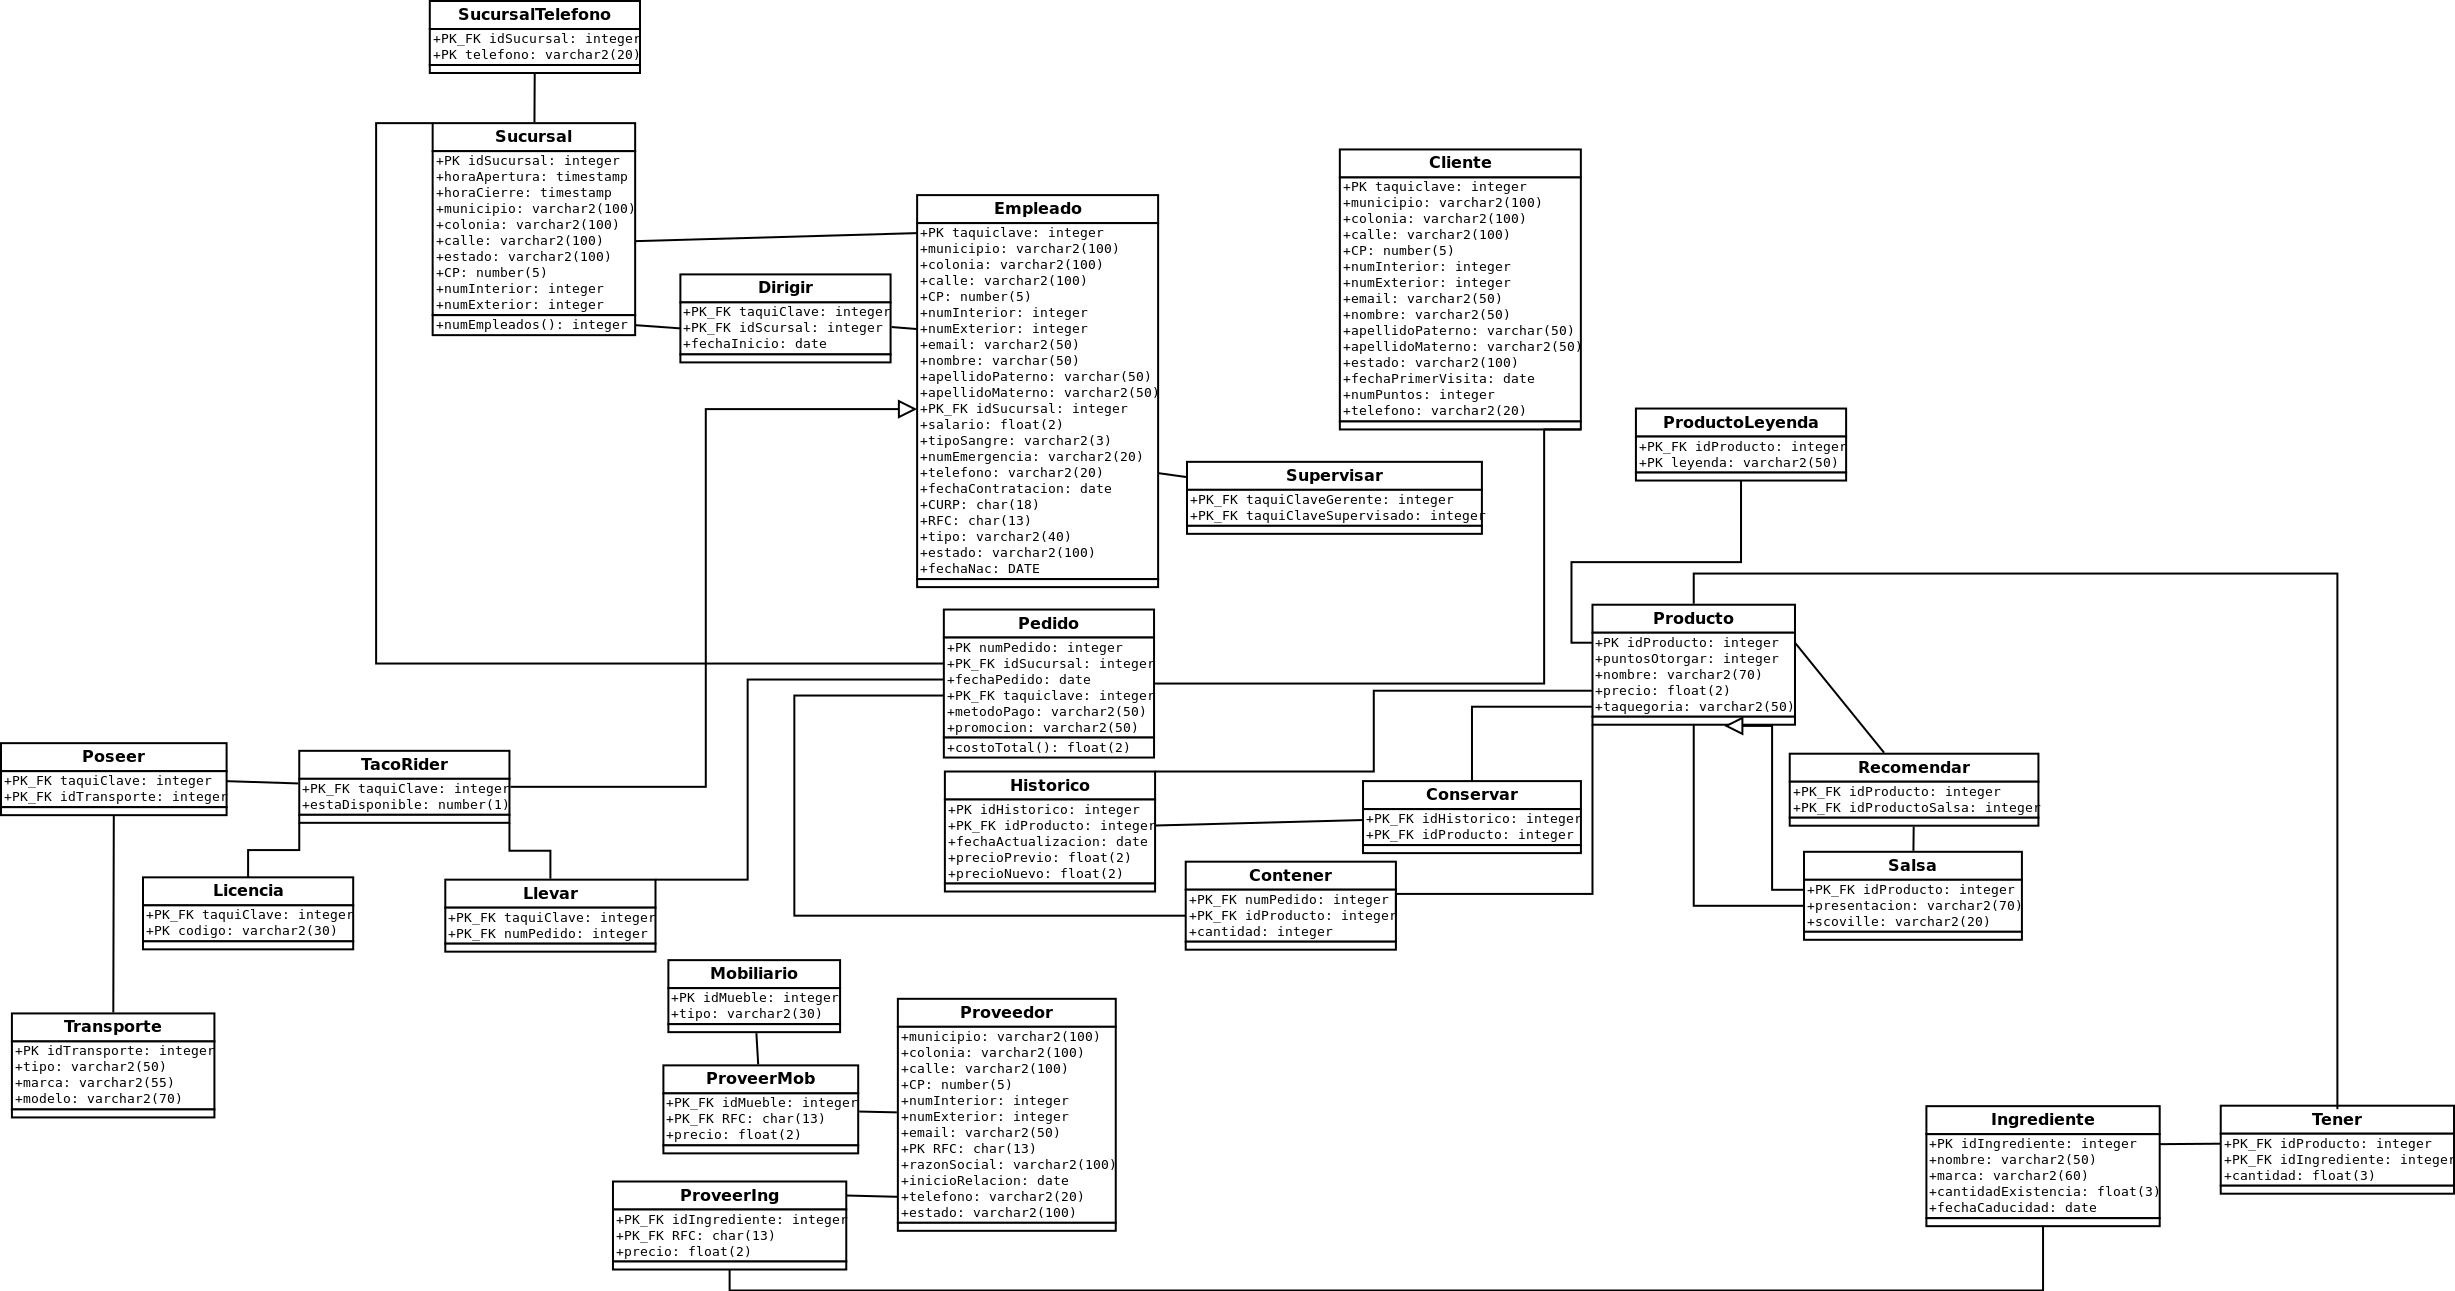
\includegraphics[scale=0.22]{UML_no_normalizado.png}
\captionof{figure}{Modelo de datos relacional obtenido a partir de la traducción del diagrama entidad-relación (ER) siguiendo el algoritmo estudiado en el curso.}
\end{minipage}
\end{center}

\end{landscape}
 \begin{thebibliography}{1}


Modelo Relacional, Avilés Rosas Gerardo. UNAM, Facultad de Ciencias,
págs. 1-29.

  \end{thebibliography}
\end{document}